\documentclass{svjour3}                     % onecolumn (standard format)

\smartqed  % flush right qed marks, e.g. at end of proof

%Essential Packages
\usepackage{graphicx,xcolor,comment,enumerate,multirow,multicol,indentfirst}

\usepackage{soul}
\usepackage{textcomp} 
\usepackage{gensymb}
\usepackage{float}
\usepackage{lineno,hyperref}
\usepackage{booktabs} 
\usepackage{calc}
\usepackage{caption}


\usepackage{authblk}

\smartqed  % flush right qed marks, e.g. at end of proof

\RequirePackage{fix-cm}
\usepackage{natbib}


\journalname{The Visual Computing}

\begin{document}

\title{An effective and friendly tool for seed image analysis}

%\titlerunning{Short form of title}        % if too long for running head

\author{Loddo A. \and
	Di Ruberto C. \and
	Vale A.M.P.G. \and
	Ucchesu M. \and
	Soares J.M. \and
	Bacchetta G.
}

%\authorrunning{Short form of author list} % if too long for running head

\institute{Loddo A., Di Ruberto C.\at
	Department of Mathematics and Computer Science, University of Cagliari, \\
	via Ospedale 72, 09124 Cagliari, Italy. \\
	\email{andrea.loddo@unica.it}
	\and
	Vale A.M.P.G.\at
	Escola Agrícola de Jundiaí (EAJ), Universidade Federal do Rio Grande do Norte (UFRN), \\
	Rodovia RN 160, Km 03, CEP 59280-000 Macaíba (RN), Brasil.
	\and
	Ucchesu M., Bacchetta G. \at
	Centro Conservazione Biodiversità (CCB), Dipartimento di Scienze della Vita e dell’Ambiente (DiSVA), Università degli Studi di Cagliari, \\
	Viale S. Ignazio da Laconi 13, 09123 Cagliari, Italy.\\
	\and
	Soares J.M. \at
	Universidade Federal do Rio Grande do Norte (UFRN), \\
	Rodovia RN 160, Km 03, CEP 59280-000 Macaíba (RN), Brasil.\\
	\and
	Bacchetta G. \at
	Hortus Botanicus Karalitanus (HBK), Università degli Studi di Cagliari, \\
	Viale S. Ignazio da Laconi 11, 09123 Cagliari, Italy.\\		
}

\date{Received: date / Accepted: date}
% The correct dates will be entered by the editor

\maketitle

\begin{abstract}
	Image analysis is an essential field for several topics of life sciences, such as biology or botany. In particular, seeds analysis (e.g., fossil research) can provide significant information about their evolution, the history of agriculture, the domestication of plants, and the knowledge of diets in ancient times. This work aims to present a software that performs an image analysis by feature extraction and classification starting from images containing seeds through a brand new and unique framework. In detail, we propose two \emph{ImageJ} plugins, one capable of extracting morphological, textural, and colour characteristics from images of seeds, and another one to classify the seeds into categories by using the extracted features. The experimental results demonstrated the correctness and validity both of the extracted features and the classification predictions. The proposed tool is easily extendable to other fields of image analysis.
\end{abstract}

\keywords{image analysis, features, classification, biology, seeds, imagej}

\section{Introduction}
Thanks to its wide range of applications, image analysis plays a vital role in the scientific field, mainly in quantitative measurements. Image visualisation and analysis methods are essential for understanding various medicinal characteristics \cite{Dirub_2015}, biology, haematology \cite{Dirub_2020}, botany and other biological branches in general. This is why biological image processing techniques have become more reliable with the development of fluorescence and high-resolution microscopes, with a profound impact on biological research giving the possibility to study the structural details of biological elements, such as organisms and parts thereof.
Biologists are increasingly interested in using image analysis techniques. ImageJ \cite{ImageJ} is defined as one of the standard image analysis software, as it is freely available, platform-independent and applicable by biological researchers to quantify laboratory tests. This paper presents a software for extracting features from biological organisms belonging to Carpology, the discipline that studies spermatophyte seeds and fruits from both a morphological and a structural perspective. This is of fundamental importance for Paleobotanica, Paleoenvironmental studies and ecology if applied to remains of the past (Paleocarpology).
Instead of manual analysis, the use of image analysis techniques on seeds has the following advantages: speed up the analysis process, minimise distortions created by natural light and microscopes, automatically identify specific characteristics based on image pixel values. The four main steps of an image analysis process are pre-processing, segmentation, features extraction, and classification \cite{Gonz_2018}.
Image pre-processing techniques prepare the image before analysing it to delete possible distortions or superfluous data or highlight and improve certain important features for further processing. The next step is segmentation. It subdivides the significant regions into sets of pixels with common features such as colour, intensity, or texture. The segmentation objective is to simplify and change image representation into something more significant and easier to analyse. Features extraction from regions of interest identified by segmentation is the subsequent step. The feature can be shape, texture or color based \cite{Dirub_2015}, \cite{Dirub_2009}. The final step is classification, i.e. the association of a label with the object under examination using supervised or unsupervised machine learning methods. 
The rest of the paper is organised as follows. The following section presents state of the art on seeds image analysis. Section 3 introduces the ImageJ environment used to implement our proposed plugin, described in Section 4. The experimental evaluation and the used dataset are discussed in Section 5, and, finally, in Section 6 we give the conclusions of the work.

%%%%%%%%%%%%%%%%%%%%%%%%%%%%%%%%%%%%%%%%%%%%%%%%%%%%%%%%%%%%%%%%%%%%%%%%%%%%%%%%%%%%%%%%%%%%%%%%%%%%%%%%%%%%%%%

\section{Material and Methods}
The analysis of seeds for different purposes is one of the possible biological-image analysis processes. For example, analysis of seed fossils can provide important information about their evolution, agriculture origin, the process of domestication and knowledge of diets in ancient times. Usually, such fossils are preserved through a process of carbonization in order to avoid microbial attacks.
In \cite{Ucc2016} Ucchesu et al. carried out different carbonization experiments to reproduce the same conditions of burning of archaeological contexts in order to compare some seeds present in Sardinia, Italy, today with the presumed archaeological fossils and so classify them.
In \cite{Ucc2015} Ucchesu et al. performed a morphological comparison between archaeological seeds and recent wild seeds. This work showed how the archaeological seeds have significantly similar features compared to modern ones. Sabato et al. \cite{Sabato2015} analyzed genetic, morphological and colourimetric differences of 124 types of \emph{Cucumismelo} seed, belonging to 48 different countries. The morpho-colourimetric analysis detected two subspecies of melons, also identifying six different varieties. The work of Orr\'u et al. \cite{Orru2012} represents, instead, the first attempt to validate a morpho-colourimetric method through a direct comparison with the molecular data of the germinal plasma, showing that the 113 proposed features are adequate to discriminate similar groups. Lo Bianco et al. \cite{LoBianco2015} identified 67 different types of Italian beans (\emph{Phaseolusvulgaris L}) using morphological features. A total of 138 descriptors, including shape and texture, have been extracted from each seed using image analysis techniques. Through \emph{Linear Discriminant Analysis} \cite{Gonz_2018}, the authors performed a comparative analysis to verify the possibility of distinguishing between seeds of the same land but cultivated with different agricultural practices. Initially, it was possible to discriminate three categories of the main seeds with an accuracy of 99.1\%. Furthermore, for each of these three categories, the cultivation land has been identified with an accuracy between 94.3\% and 99.7\%.

\subsection{Dataset description}
For this study, we used an image database containing 3,386 samples of 120 plant species belonging to the \emph{Fabaceae} family.
We chose the \emph{Fabaceae} family because it is one of the most prominent families and shows significant variability in their seeds' size and colour. 
All samples come from the base collection in the Germplasm Bank of Sardinia (BG-SAR), University of Cagliari, Italy.
During the acquisition, the operators arranged the seeds on the flatbed scanner, separating them from each other in order to avoid overlapping. Then the area occupied by the seeds has been covered with a tray lined with a blue background for the digital image, as shown in Figure \ref{Acquisition}. The acquisition process used a minimum resolution of 400 dpi and the resulting image saved in the Joint Photographic Experts Group (Jpeg) format with a resolution of $2125\times2834$ \cite{Loddo20}.

\begin{figure}[tbp]
	\centerline{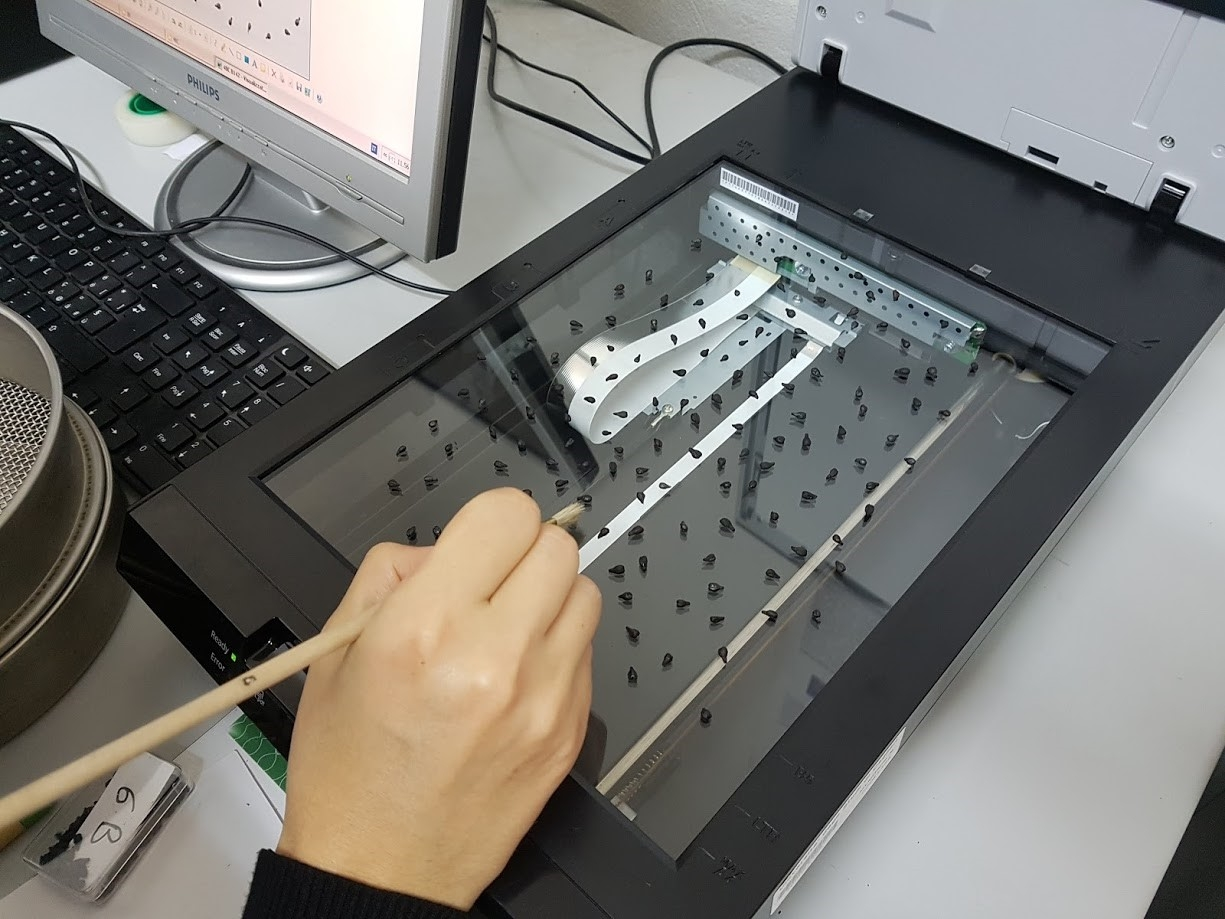
\includegraphics[scale=0.25]{Acquisition.jpg}}
	\caption{Seeds acquisition on the flatbed scanner for the \emph{Fabaceae} dataset.}
	\label{Acquisition}
\end{figure}

For the classification task, we selected the more numerous species.
Next, we applied a preprocessing procedure. 
In particular, the collectors acquired these seeds' images on different backgrounds of various shades of blue. Consequently, it helps us to find the best images to extract crops of single seeds to classify. Figure \ref{Sardinia} shows two sample images from the \emph{Fabaceae} database.

\begin{figure}[tbp]
	\centerline{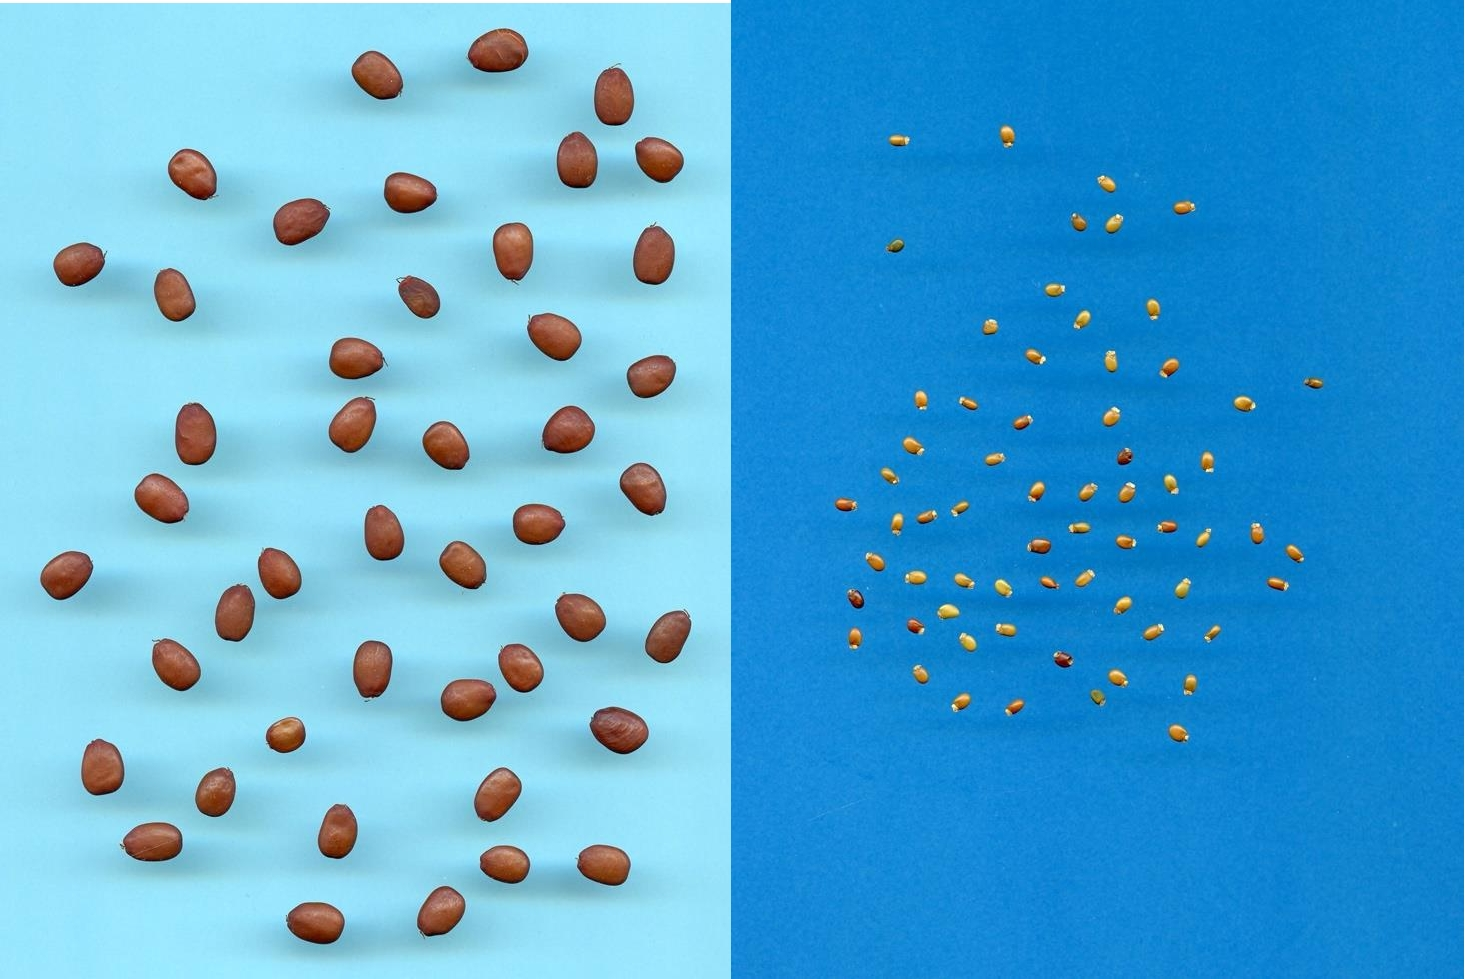
\includegraphics[scale=0.5]{Sardinia.jpg}}
	\caption{Examples of seeds images present in the \emph{Fabaceae} dataset.}
	\label{Sardinia}
\end{figure}

\subsection{ImageJ platform}
ImageJ \cite{ImageJ} is open-source software for digital image processing, designed initially by Wayne Rasband from the National Institute of Health of the United States. It is written in Java language, and it runs as an online applet or offline with an installed Java Virtual Machine (JVM). The source code is publicly available and open to new contributions for the ImageJ community. ImageJ allows viewing, analyzing, modifying, processing, saving, printing grayscale images (8-bit, 16-bit, and 32-bit) and color images (8-bit and 24-bit); the supported formats are TIFF, JPEG, GIF, BMP, DICOM, FITS, and RAW. It was designed with an open architecture extendable with two kinds of extension, \emph{Java plugins}, and recordable \emph{macros}. Most of the existing plugins already permit to face some image processing and analysis issues.
ImageJ allows the extraction of Region of Interest (ROI) pixel-wise or object-segmented statistics. It is also possible to measure distances and angles, generate and visualize intensity histograms and draw profile lines (between defined points). ImageJ supports many standard image processing transformations, such as logical and arithmetic operations between images, brightness and contrast adjustment, convolution, Fourier analysis, smoothing, contour detection, median filtering, and mathematical morphology \cite{Gonz_2018}. It is also possible to perform geometric transformations such as scaling, rotation, and reflection.

The interface of ImageJ is straightforward and intuitive even for people without advanced computer and image analysis skills. 
Basically, the software is condensed in its menu bar that contains all the options, as shown in Figure \ref{ImageJ_Interf}.

\begin{figure}[!t]
	\centerline{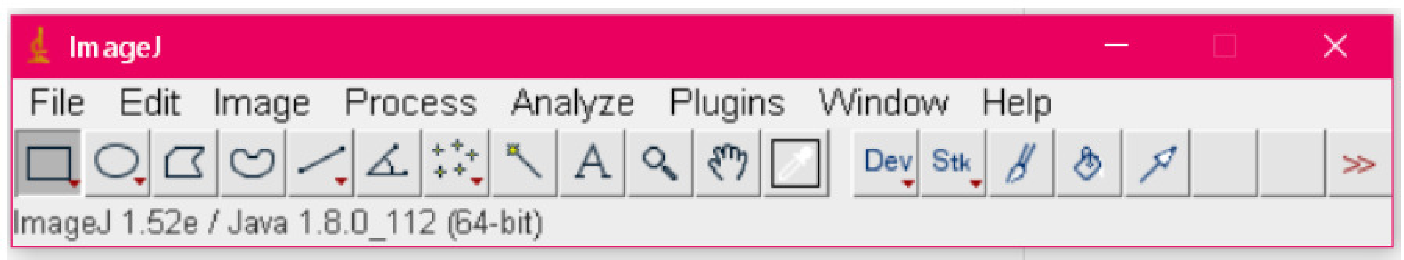
\includegraphics[scale=0.37]{Fig1.pdf}}
	\caption{ImageJ main interface.}
	\label{ImageJ_Interf}
\end{figure}
Basic operations, like file opening or simple editing options (File and Edit options) and more complex ones, such as segmentation operations, image enhancement, noise reduction, object counting, filtering, and other options ("Image," "Process," "Analyze" and "Plugins"), are accessible from the main menu.
Moreover, the toolbar contains several options to select regions or shapes in the image. 
The status bar shows the current pixel's coordinates and values when the cursor is over the image. Simultaneously, whether a filter operation is performed on the image, the status bar displays the execution time and the processing speed in $pixels / second$.
The progress bar, shown on the right-hand side of the status bar, shows the processing progress.

ImageJ allows an extension of its functionalities through additional components, like plugins and macros. The plugins require Java language, while macros require Java-like language. Plugins are generally faster and more flexible; on the other hand, macros are simpler to write and debug, but they are heavier than the plugins computationally. It is the main reason that led plugins to play a fundamental role in functionality extensions and ImageJ itself since it implements a large part of its functionality with internal plugins.

\subsubsection{ImageJ's logical structure}
ImageJ presents a very extensive and complex class diagram.
\emph{IJ} is the main class of the framework: any processing starts from it, and consequently, all the other classes extend it or are part of \emph{ij}.* package. It takes an image in input and returns an object of the \emph{ImagePlus} type, ready for its analysis.
The created \emph{ImagePlus} object contains an object of the abstract \emph{ImageProcessor} class, which stores image data in 2D and provides methods for processing.
The \emph{GenericDialog} and \emph{ResultsTable} classes respectively manage input and output data. The first one allows the user to specify preferences and select options via several checkboxes, text boxes, and lists, while the second one shows the output results in tabular form. Moreover, the \emph{ROI} class permits the processing of an image's objects.
This class includes several parameters and methods and is often associated with an object of type \emph{ImageStatistics} that consists of a series of measurements calculated on the ROI. The \emph{ROI} class uses the classes\emph{Polygon Java } and its subclasses to determine the points which constitute an area of interest. The \emph{Analyzer} class returns an object based on particular options that analyze the image. An object of type \emph{ParticleAnalyzer} works in the same manner even though it analyses all the regions in an image one-by-one rather than the whole image. 
The class \emph{Histogram} provides an image histogram on a ROI. 
\emph{ChannelSplitter} returns a vector containing three \emph{ImagePlus}, each one corresponding to a single RGB (Red, Green, Blue) channels.
In the next section, we detail our proposed plugin structure, based on the \emph{ParticleAnalyzer}'s logical structure.

%%%%%%%%%%%%%%%%%%%%%%%%%%%%%%%%%%%%%%%%%%%%%%%%%%%%%%%%%%%%%%%%%%%%%%%%%%%%%%%%%%%%%%%%%%%%%%%%%%%%%%%%%%%%%%%

\section{A tool for seed image analysis}
ImageJ allows the realisation of new plugins, e.g., dealing with specific problems in the image analysis field or computing new features in different contexts.
Among the state-of-the-art, different plugins already exist and can extract features from seeds images, even though they are general-purpose. One of them is \emph{Particles8} \cite{Landini}, created by Gabriel Landini in 2005, with the last update in 2010. It provides the extraction of morphological features from binary images. Consequently, it does not provide the extraction of textural and colour features.
To simplify the botanists' seed analysis procedures, we followed their indications, and we realised a brand new plugin exclusively with \emph{ImageJ} classes without using any external plugins and increasing its extensibility. The proposed tool allows the extraction and classification of features and can be used in many other application domains.

\subsection{A plugin for feature extraction from seeds image}
\label{seeds_analyser}
\emph{SeedsAnalyser} is the plugin for feature extraction proposed in this work and needs a minimal number of user interactions. It aims to identify and analyse multiple seeds represented in a digital image. The input is a single image acquired with a quasi-uniform blue background.
The plugin is also able to analyse all the images in a specific folder at the same time. Each image can present a blue background in a wide range of tones, varying from a very light blue to a very dark navy blue. After the acquisition, the image is preprocessed for the correct separation of the regions of interest, namely the single seeds. 
It is possible to isolate the Blue value of the RGB images to get pure masks as the dataset backgrounds are all in various shades of blue (see Figure \ref{Sardinia_Masks}), as indicated in our previous work \cite{Loddo20}. 
Creating a single seed dataset from the original database is possible thanks to different backgrounds of various blue shades. It allowed finding the best images to work on and making the binary masks to extract the single seeds just by an automatic thresholding procedure.
During the acquisition, the seeds were well spaced from each other. Therefore the bounding box of each region allowed the creation of a single seed image for analysis quickly.
From the \emph{Fabaceae} dataset, we selected the images containing the most numerous samples per species for 23 different species and nearly 2000 seeds.
We discarded some species due to the low sharpness and too small size of the seeds. Figures \ref{Sardinia_Masks} and \ref{Sardinia_Crops} show an original sample image with its derived binary mask and some seed images extracted from it, respectively. 
\begin{figure}[htbp]
	\centering
	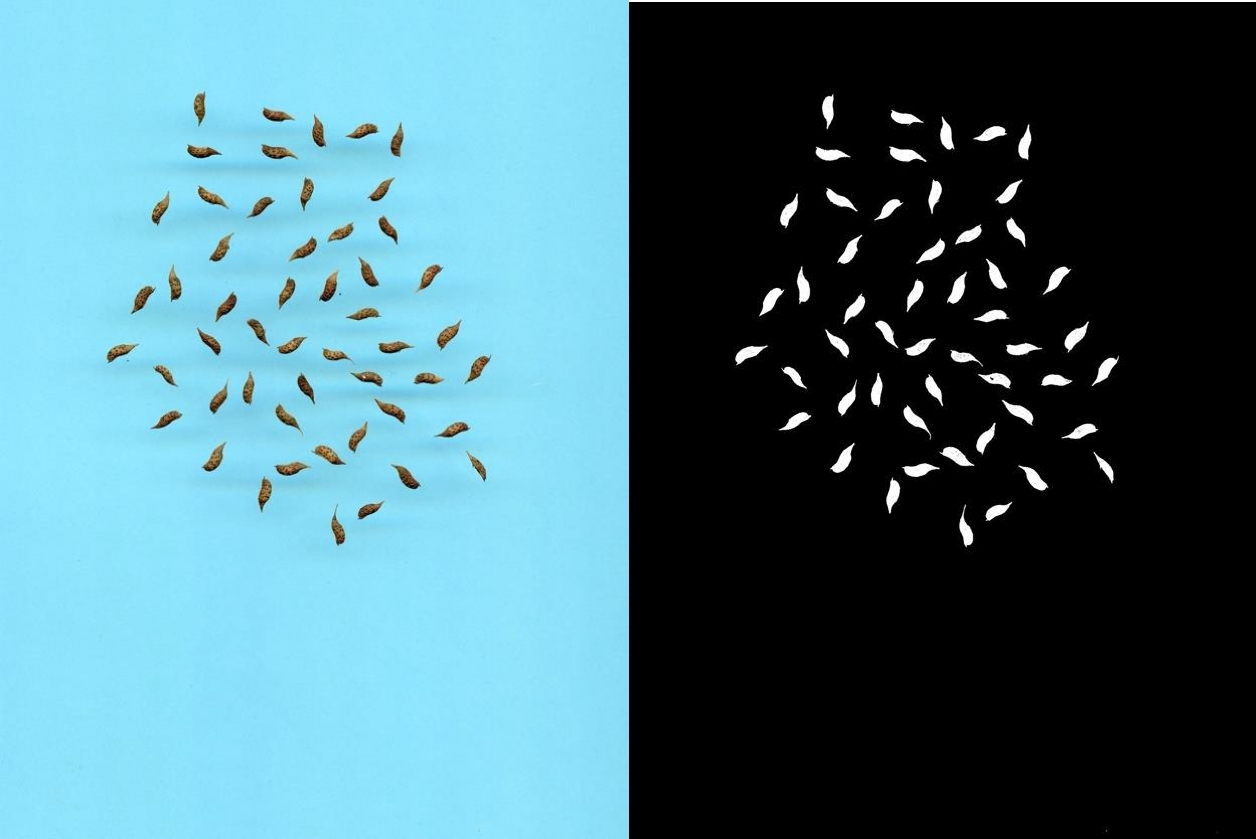
\includegraphics[scale=0.6]{SardiniaMasks.jpg}
	\caption{Example of an image from the \emph{Fabaceae} database and its derived binary mask.}
	\label{Sardinia_Masks}
\end{figure}

\begin{figure}[htbp]
	\centering
	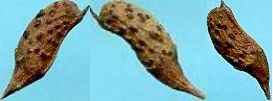
\includegraphics[scale=0.4]{Sardinia_crops.jpg}
	\caption{Some examples of seed images extracted from the image of Figure \ref{Sardinia_Masks} of the \emph{Fabaceae} database.}
	\label{Sardinia_Crops}
\end{figure}

Once the images have been preprocessed, i.e. segmented by automatic thresholding, and the unique image is ready to be analyzed, the plugin requires the selection of some key parameters. They improve the research and detection of the regions of interest, specifically the minimum and maximum area size, measured in square pixels and, if wanted, a specific circularity of the objects, by default ranging from 0 to 1.
Finally, the users can choose the features of interest from the "Feature" window, as shown in Figure \ref{fig:features_selection}.

\begin{figure}[htbp]
	\centering
	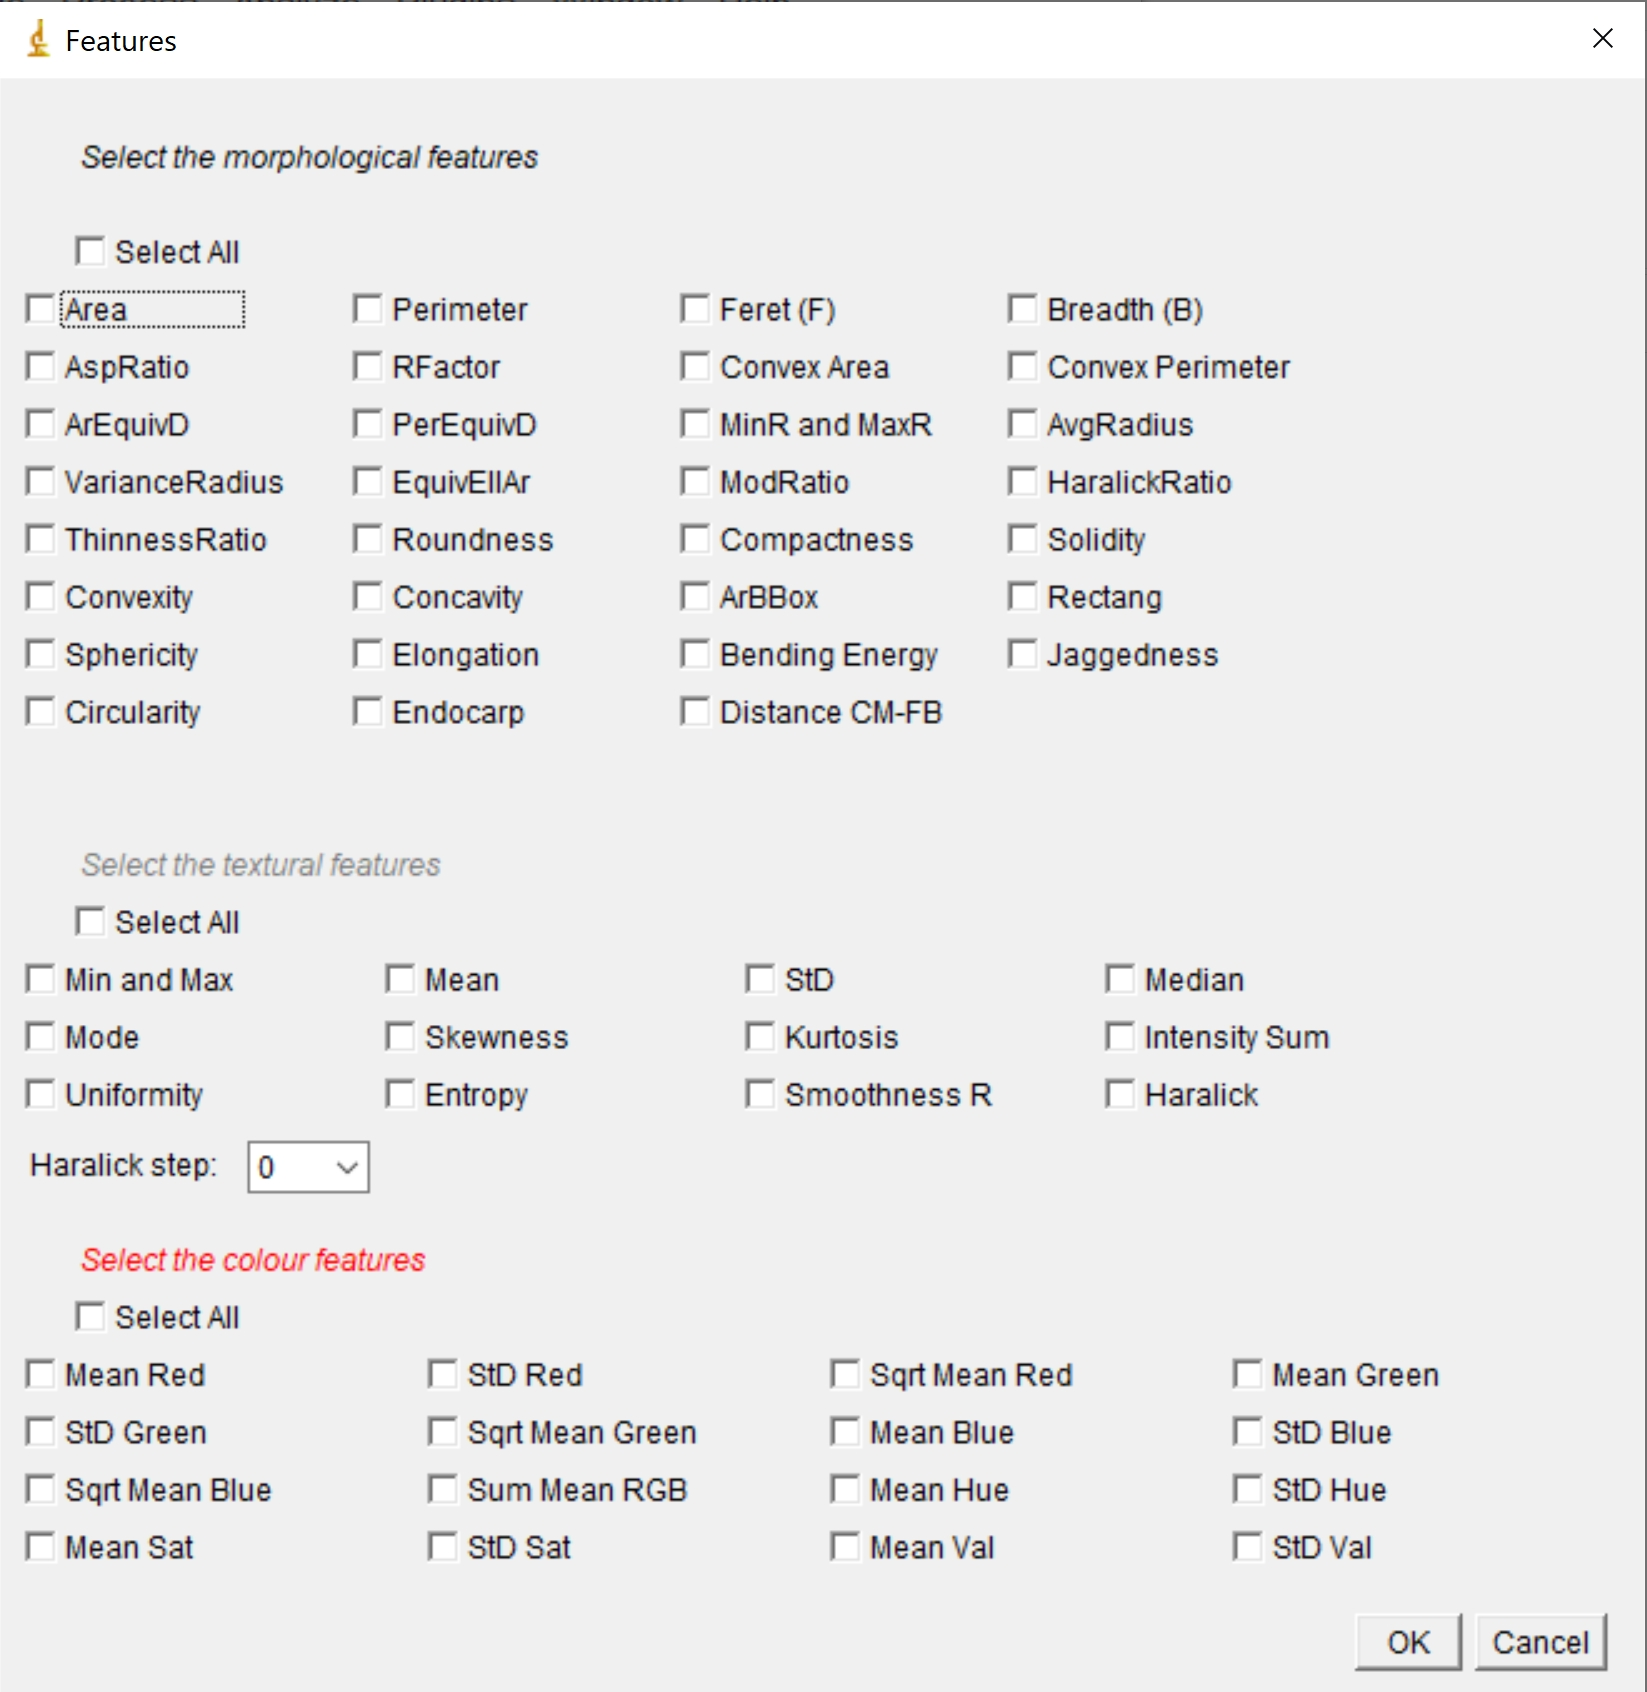
\includegraphics[height=0.35\textheight]{Features_selection.jpg}
	\caption{\label{fig:features_selection}Window for feature selection.}
\end{figure}

\emph{SeedsAnalyser} implements up to 64 features. In particular, 32 are morphological, 16 textural and 16 colour intensity values. It is crucial to notice that, among the texture features, Haralick's GLCM \cite{Haralick73}, which describes the pairwise arrangement of pixels with the same grey-level, was used in this study to extract information of local similarities. All of them permits their computation with the typical four different degrees: 0\degree, 45\degree, 90\degree, 135\degree. More precisely, we extracted the following second-order statistics from GLCM: energy, contrast, correlation and homogeneity.
ImageJ already contains a plugin that works in a way similar to \emph{Seeds Analyser}, even though it only offers 18 features, and it does not have a multi-image workflow.
To sum up, after the initial preprocessing step, our plugin can detect each single seed present in the original RGB image from which the user can select the morphological, textural and colour features to extract. Table \ref{table:morph} and Table \ref{table:gray} present the implemented morphological and textural features, respectively, and their relative descriptions, while Table \ref{table:col} describes the computed features of the RGB and HSV colour spaces.

\begin{table*}[htbp]
	\caption{Morphological features from binary image}
	\centering 
	\footnotesize
	\scalebox{0.90}{
		\begin{tabular}{ l l } 
			\hline
			\textbf{Feature} & \textbf{Description} \\
			\hline
			\emph{Area} & Seed area (in pixels) \\
			\emph{Perimeter} & Length of the seed contour \\
			\emph{Feret} & Longest traceable diameter with two points of the seed's outline as endpoints, called Lenght\\
			\emph{Breath} & Length of longest traceable axis perpendicular to the Feret, also called Width\\
			\textit{AspRatio} & \textit{Feret}/\textit{Breadth}, also called eccentricity or rectangularity ratio\\
			\emph{ConvexArea} & Area of the convex polygon drawn between the external points of the region\\
			\emph{ConvexPerimeter} & Perimeter of the convex polygon \\
			\textit{RFactor} & Shape factor, defined as $CovenxArea/(Feret\times pi)$\\
			\textit{ArEquivD} & Diameter of the circle with equivalent area of the region, defined as $\sqrt{4/\pi \times Area}$  \\
			\textit{PerEquivD} & Diameter of the circle having the same perimeter of the region, $Area/\pi$ \\
			\textit{MinR} and \textit{MaxR} & Radii of the inscribed and the enclosing circles centred at the center of mass\\
			\textit{AvgRadius} & Average length of the radii calculated starting from the center of mass \\
			\textit{VarianceRadius} & Variance of radii \\ 
			\textit{EquivEllAr} & Area of the ellipse having \emph{Feret} and \emph{Breadth} as axes \\
			\textit{Modification Ratio} & Shape measure, defined as $(2 \times MinR)/Feret$ \\
			\textit{Haralick Ratio} & Ratio between the average and the standard deviation of the radii \\
			\textit{ThinnessR} & Thinness Ratio, also called shape, given by $ Perimeter^2 / Area $ \\
			\textit{Roundness} & Measure of roundness, defined as $4 \times Area/(\pi \times Feret^2)$ \\
			\textit{Compactness} & Measure of compactness, expressed by $\sqrt{4/\pi \times Area/Feret}$  \\
			\textit{Solidity} & Measure of solidity, defined as $Area/ConvexArea$ \\
			\textit{Convexity} & Measure of convexity, also called roughness, defined as $ConvexPerimeter/Perimeter$ \\
			\textit{Concavity} & Measure of concavity, defined as $ConvexArea$ - $Area$\\
			\textit{ArBBox} & Area of the bounding box containing the region \\
			\textit{Rectangularity} & Also called extent, defined as $Area / ArBBox$ \\
			\textit{Sphericity} & Also called radius ratio, expressed by $MinR/MaxR$ \\
			\textit{Elongation} & Inverse of the circularity, defined as $Perim^2 / (4 \times \pi \times Area) $\\
			\textit{Bending Energy} & Defined as the sum of the squared curvature along the entire contour \\
			\textit{Jaggedness} & Measure representing if a seed is "serrated", defined as $(2\times \sqrt{\pi\times Area})/Perimeter$ \\
			\textit{Circularity} & Also called shape factor, obtained by $2\times \pi \times Area/Perimeter^2$ \\
			\textit{Endocarp} & Number of pixels forming the seed endocarp\\
			\textit{FBtoCM} & Distance between the intersection coordinates of seed length and width and center of mass \\
			\hline
	\end{tabular}}
	\label{table:morph}
\end{table*}

\begin{table*}[htbp]
	\caption{Texture features from grayscale image}
	\centering 
	\footnotesize
	\scalebox{0.95}{
		\begin{tabular}{ l l } 
			\hline
			\textbf{Feature} & \textbf{Description} \\
			\hline
			\textit{Min} and \textit{Max} & Minimum and maximum gray value in the region \\
			\textit{Mean} & Average gray value in the region\\
			\textit{StD} & Intensity standard deviation as contrast measure \\
			\textit{Median} & Median of the gray values \\
			\textit{Mode}  & Mode of the gray values \\
			\textit{Skewness} & Measure of the symmetry of the graylevel histogram around the average value \\
			\textit{Kurtosis} & Measure of the "tailedness" of the graylevel histogram \\
			\textit{Intensity Sum} & Sum of the gray values of the region \\
			\textit{Uniformity} & Maximum when all the gray levels in the histogram are equal \\
			\textit{Entropy} & Measure of variability of grey level distribution \\
			\textit{Smoothness R }& Measure of smoothness \\ 
			\textit{Haralick} & GLCM's computed second-order statistics (Energy, Contrast, Correlation, Homogeneity) \\
			\hline
	\end{tabular}}
	\label{table:gray}
\end{table*}

\begin{table}[htbp]
	\caption{Color features from RGB and HSV color spaces}
	\centering 
	\footnotesize
	\begin{tabular}{ l l } 
		\hline
		\textbf{Feature} & \textbf{Description} \\
		\hline
		\textit{Mean Red (MR) }& Average of Red channel values \\
		\textit{StD Red} & Standard deviation of Red channel values \\
		\textit{SqrtMean Red} & Square root of the mean value for Red channel  \\
		\textit{Mean Green (MG)} & Average of Green channel values \\
		\textit{StD Green} & Standard deviation of Green channel values \\
		\textit{SqrtMean Green} & Square root of the mean value for Green channel \\
		\textit{Mean Blue (MB)} & Average of Blue channel values \\
		\textit{StD Blue} & Standard deviation of Blue channel values \\
		\textit{SqrtMean Blue} & Square root of the mean value for Blue channel \\
		\textit{Mean RGB} & \( \frac{MR + MG + MB}{3} \)\  \\ 
		\textit{Mean Hue} & Average tone of Hue channel \\
		\textit{StD Hue} & Standard deviation of Hue channel values \\			
		\textit{Mean Sat} & Average tone of Saturation channel \\
		\textit{StD Sat} & Standard deviation of Saturation channel values \\
		\textit{Mean Val} & Average tone of Value channel \\
		\textit{StD Val} & Standard deviation of Value channel values \\
		\hline
	\end{tabular}
	\label{table:col}
\end{table}

\subsection{A plugin for feature classification}
\label{feature_classifier}
Up to now, we have obtained the features for each seed from \emph{SeedsAnalyser} \ref{seeds_analyser}, and they can now be fed to the classification plugin, called \emph{SeedsClassifier}.
It offers four different classifiers, namely kNN, Naive Bayes, Random Forest and SVM. Weka \cite{Weka} includes all of them; therefore, they can be imported individually from their respective packages. All classifiers belong to their java class, where they implement the Classifier interface responsible for defining and realising the classification procedure.
At the plugin's start, the user can choose whether to load an existing model or start a new training phase on new data. If the user chooses to proceed from scratch, i.e. also with the training phase, the user will be asked to enter the ARFF file's name with the training dataset. For practical reasons, this file must be located in the main folder of the framework. The predictions will be displayed in a window called Predictions.
As we mentioned earlier, \emph{SeedsClassifier} plugin allows for the use of four classification algorithms. We now briefly describe how they operate and differ from each other.
In general, Naive Bayes classifiers are probabilistic models that use Bayes' theorem with strict independence assumptions between the features. 
%
KNN uses the \textit{k} closest training samples in the dataset as input and then uses a neighbour voting strategy to rank and classify new objects. Generally speaking, the larger k is, the more the noise associated with classification is reduced, but class recognition becomes more difficult. 
%
The Support Vector Machine (SVM) is a non-probabilistic binary linear classifier that categorises objects by mapping examples to points in space to maximise the width of the distance between categories. 
%
Finally, Random Forest is made up of many individual decision trees that work together to form an ensemble. Each tree predicts a class, and the class with the most votes is the model prediction. However, there is a need for each tree not to correlate with the others. This would jeopardise the classifier's final decision. In this way, the trees protect each other from their errors.
%
Given our feature spaces' abundance and diversity, we choose these classifiers to ensure classification accuracy, flexibility, and data adaptation.

%%%%%%%%%%%%%%%%%%%%%%%%%%%%%%%%%%%%%%%%%%%%%%%%%%%%%%%%%%%%%%%%%%%%%%%%%%%%%%%%%%%%%%%%%%%%%%%%%%%%%%%%%%%%%%%

\section{Experimental results} 
We now describe the experimentations conducted to verify the correctness of the features extracted from \emph{SeedsAnalyser} using the classification plugin.
We selected the images containing the most numerous samples per species from the \emph{Fabaceae} database, for a total of 23 different ones: 
\emph{Amorpha}, \emph{Anagyris}, \emph{Anthyllis barba jovis}, \emph{Anthyllis cytisoides}, \emph{Astragalus glycyphyllos}, \emph{Calicotome}, \emph{Caragana}, \emph{Ceratonia}, \emph{Colutea}, \emph{Cytisus purgans}, \emph{Cytisus scoparius}, \emph{Dorycnium pentaphyllum}, \emph{Dorycnium rectum}, \emph{Hedysarum coronarium}, \emph{Lathyrus aphaca}, \emph{Lathyrus ochrus}, \emph{Medicago sativa}, \emph{Melilotus officinalis}, \emph{Pisum}, \emph{Senna alexandrina}, \emph{Spartium junceum}, \emph{Trifolium}, \emph{Vicia faba}, for a total of 1988 seeds.
A sample of each species is shown in Figure \ref{Sardinia_samples}, while Table \ref{Sardinia_tab} reports the number of samples for each species.

\begin{figure}[htbp]
	\centering
	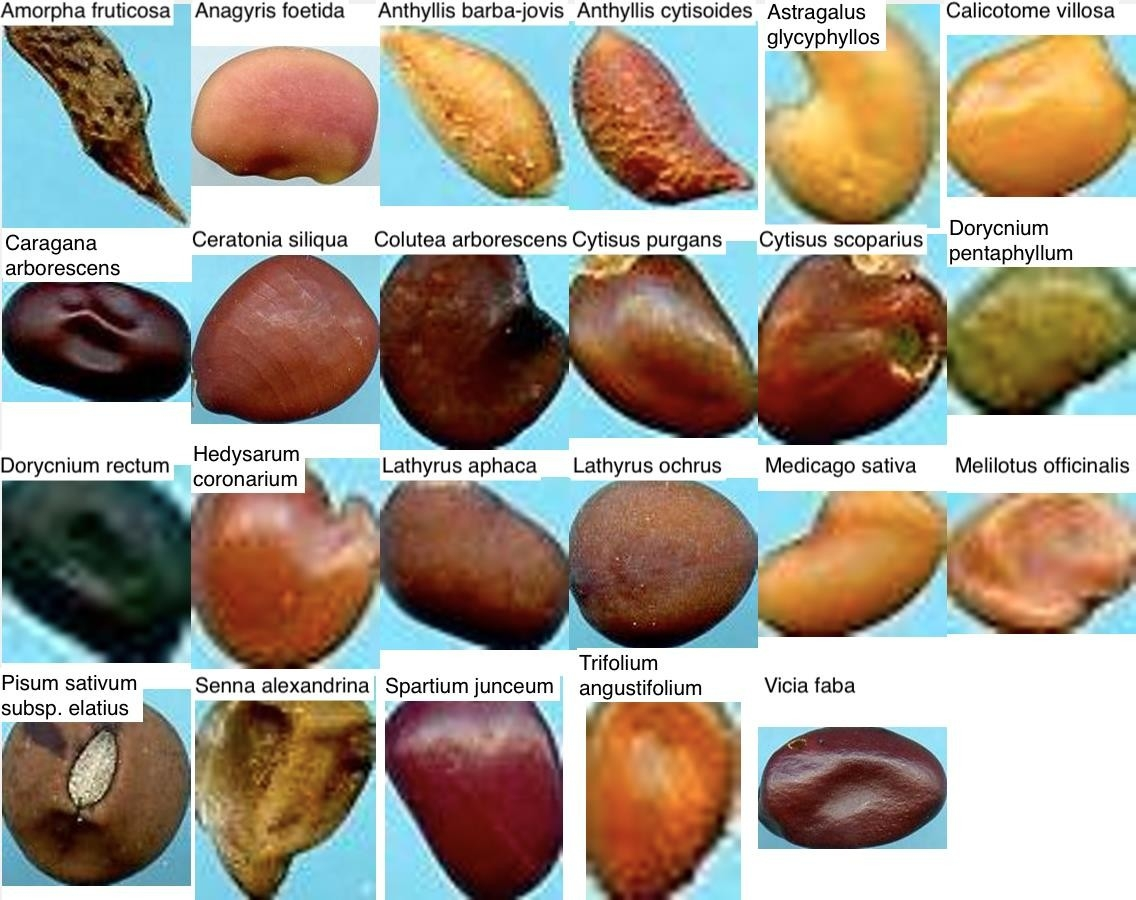
\includegraphics[scale=0.65]{Sardinia_samples.jpg}
	\caption{A sample of seed for each species present in the \emph{Fabaceae} dataset.}
	\label{Sardinia_samples}
\end{figure}

\begin{table}[htbp]
	\centering
	\small
	\hspace{0.05cm}
	\begin{tabular}{lc}
		\hline
		\textbf{Species} & \textbf{Num. of samples} \\
		\hline
		\emph{Amorpha} & 51 \\
		\emph{Anagyris} & 29 \\
		\emph{Anthyllis barba jovis} & 51 \\
		\emph{Anthyllis cytisoides} & 29 \\
		\emph{Astragalus glycyphyllos} & 50 \\
		\emph{Calicotome} & 32 \\
		\emph{Caragana} & 36 \\
		\emph{Ceratonia} & 45 \\
		\emph{Colutea} & 42 \\
		\emph{Cytisus purgans} & 44 \\
		\emph{Cytisus scoparius} & 65 \\
		\emph{Dorycnium pentaphyllum} & 42 \\
		\emph{Dorycnium rectum} & 236 \\
		\emph{Hedysarum coronarium} & 208 \\
		\emph{Lathyrus aphaca} & 52 \\
		\emph{Lathyrus ochrus} & 46 \\
		\emph{Medicago sativa} & 116 \\
		\emph{Melilotus officinalis} & 176 \\
		\emph{Pisum} & 121 \\
		\emph{Senna alexandrina} & 194 \\
		\emph{Spartium junceum} & 109  \\
		\emph{Trifolium} & 183 \\
		\emph{Vicia faba} & 31 \\
		\hline
	\end{tabular}
	\caption{\emph{Fabaceae} dataset description.} 
	\label{Sardinia_tab}
\end{table}

As described in Sec. \ref{seeds_analyser} we have implemented and extracted three categories of handcrafted features from the seeds: morphological structure, texture information, and colour intensity values, for a total amount of 64 descriptors. Afterwards, we provided them as inputs to four different classification models, namely kNN, Naive Bayes, Random Forest, and Support Vector Machine, using our plugin \emph{SeedsClassifier}, based on Weka package tool \cite{Weka}. 

To ensure training set heterogeneity, we trained each classifier with 10-fold cross-validation, and for each case, we selected the model with the largest area under the ROC curve (AUC). 

The performance measures used to quantify each classification model's performance are specificity, sensitivity, and accuracy. 
The specificity (Spec) measures the proportion of negatives that are correctly identified (also called true negative rate). The sensitivity (Sen) measures the proportion of positives that are correctly identified (also called true positive rate).
The third measure is the accuracy (Acc), defined as the correctly labelled instances' ratio to the whole pool of instances. 
Finally, as we face a multi-class imbalanced problem, we also applied three of the most common global metrics for multi-class imbalance learning to evaluate the classifier's performance \cite{Alejo2013}. The used measures are the macro average geometric (MAvG), defined as the geometric average of the partial accuracy of each class, the mean F-measure (MFM) and the macro average arithmetic (MAvA), defined as the arithmetic average of the partial accuracies of each class. 

We performed several experiments for each classifier. In particular, we tested the descriptors categories both alone and in combination with the others to understand if there is the best descriptor category for this task. Finally, we use the \emph{SeedsClassifier} plugin to classify each category with the chosen classifiers.

Tables \ref{Table_classification_kNN}, \ref{Table_classification_Bayes}, \ref{Table_classification_RF}, \ref{Table_classification_SVM} show all the classification results on the analysed dataset.
In detail, the kNN classifier shows high results with colour features category alone, outperforming the remaining. Surprisingly, the combination of all categories does not reach the best metric results with this classifier.
Random Forest classifier substantially confirms the trend brought by the colour feature category. It outperforms every other combination, even against the remaining classifiers. However, the combination of all categories produced excellent results with the Random Forest model.
Naive Bayes and SVM classifiers produced satisfactory results using all categories, which results in the best one for both classifiers. Contrary to kNN and Random Forest results, the colour category alone did not produce good results in these last two cases.
To sum up, the Random Forest classifier produced the best performance and is the only one to exceed 90\% both in metrics and in categories combination. It confirms its outstanding versatility in this twenty-three-class scenario. 
Finally, we can say that combining all the three feature categories produces excellent results in most cases and satisfactory on average.

\begin{table}[htbp]
	\centering
	\caption{Results using every possible combination of classic descriptors and kNN.}
	\label{Table_classification_kNN}
	\begin{tabular}{lcccccc}
		\toprule
		Descriptors    &  Acc  & Spec  &  Sen  & MAvG  &  MFM  & MAvA  \\ \midrule
		Morphological & 20.95 & 23.18 & 17.10 & 9.94 & 18.59 & 23.18 \\
		Texture & 16.41 & 20.52 & 16.97 & 10.91 & 16.36 & 20.52 \\
		Colour & 80.54 & 76.59 & 74.70 & 74.72 & 75.15 & 76.59 \\
		Morphological+Texture & 31.25 & 27.57 & 22.17 & 13.73 & 23.62 & 27.57 \\
		Morphological+Colour & 45.13 & 41.63 & 33.47 & 27.08 & 35.34 & 41.63 \\
		Texture+Colour & 68.61 & 62.33 & 58.44 & 57.74 & 59.73 & 62.33 \\
		All & 71.68 & 69.54 & 63.02 & 65.60 & 65.17 & 69.54 \\ \bottomrule
	\end{tabular}
\end{table}

\begin{table}[htbp]
	\centering
	\caption{Results using every possible combination of classic descriptors and Naive Bayes.}
	\label{Table_classification_Bayes}
	\begin{tabular}{lcccccc}
		\toprule
		Descriptors    &  Acc  & Spec  &  Sen  & MAvG  &  MFM  & MAvA  \\ \midrule
		Morphological & 62.42 & 59.88 & 62.04 & 53.34 & 59.68 & 59.88 \\
		Texture & 48.19 & 47.59 & 45.84 & 39.58 & 43.43 & 47.59 \\
		Colour & 65.21 & 60.75 & 62.25 & 55.02 & 57.93 & 60.75 \\
		Morphological+Texture & 76.81 & 73.00 & 75.10 & 68.51 & 72.89 & 73.00 \\
		Morphological+Colour & 84.36 & 81.66 & 84.43 & 79.22 & 82.35 & 81.66 \\
		Texture+Colour & 79.33 & 76.14 & 79.15 & 72.81 & 75.74 & 76.14 \\ 
		All & 85.16 & 81.78 & 84.82 & 79.68 & 82.76 & 81.78 \\ \bottomrule
	\end{tabular}
\end{table}

\begin{table}[htbp]
	\centering
	\captionsetup{width=.9\textwidth}
	\caption{Results using every possible combination of classic descriptors and Random Forest.}
	\label{Table_classification_RF}
	\begin{tabular}{lcccccc}
		\toprule
		Descriptors    &  Acc  & Spec  &  Sen  & MAvG  &  MFM  & MAvA  \\ \midrule
		Morphological & 40.48 & 46.85 & 29.13 & 37.96 & 27.58 & 46.85 \\
		Texture & 72.03 & 65.88 & 60.38 & 62.09 & 61.17 & 65.88 \\
		Colour & 94.27 & 94.85 & 91.05 & 94.67 & 92.52 & 94.85 \\
		Morphological+Texture & 89.64 & 90.67 & 81.96 & 90.09 & 83.79 & 90.67 \\
		Morphological+Colour & 92.71 & 93.57 & 88.94 & 93.36 & 90.67 & 93.57 \\
		Texture+Colour & 92.05 & 92.41 & 87.16 & 92.21 & 89.07 & 92.41 \\ 
		All & 93.76 & 94.55 & 89.75 & 94.37 & 91.39 & 94.55 \\ \bottomrule
	\end{tabular}
\end{table}

\begin{table}[htbp]
	\centering
	\caption{Results using every possible combination of classic descriptors and SVM.}
	\label{Table_classification_SVM}
	\begin{tabular}{lcccccc}
		\toprule
		Descriptors    &  Acc  & Spec  &  Sen  & MAvG  &  MFM  & MAvA  \\ \midrule
		Morphological & 79.83 & 80.26 & 71.33 & 79.46 & 73.23 & 80.26 \\
		Texture & 29.09 & 46.28 & 21.13 & 34.11 & 16.91 & 46.28 \\
		Colour & 78.74 & 75.28 & 67.83 & 72.42 & 67.88 & 75.28 \\
		Morphological+Texture & 66.05 & 59.81 & 51.10 & 52.83 & 52.44 & 59.81 \\
		Morphological+Colour & 83.60 & 83.10 & 76.70 & 81.65 & 78.88 & 83.10 \\
		Texture+Colour & 84.51 & 84.99 & 77.73 & 84.15 & 78.81 & 84.99 \\
		All & 85.66 & 83.85 & 78.88 & 82.56 & 80.58 & 83.85 \\ \bottomrule
	\end{tabular}
\end{table}

%%%%%%%%%%%%%%%%%%%%%%%%%%%%%%%%%%%%%%%%%%%%%%%%%%%%%%%%%%%%%%%%%%%%%%%%%%%%%%%%%%%%%%%%%%%%%%%%%%%%%%%%%%%%%%%

\section{Conclusions}
We presented a software that performs an image analysis by feature extraction and classification from images containing seeds through a brand new unique, and easy-to-use framework. In detail, we propose two \emph{ImageJ} plugins, one capable of extracting morphological, textural and colour characteristics from images of seeds, and another one to classify the seeds into categories by using the extracted features. 
Moreover, we analysed and reported the performances of several categories of descriptors for seed images with four different classifiers, using an image database containing 3,386 samples of 120 plant species belonging to the \emph{Fabaceae} family. 
In general, some aspects can strongly influence both the feature extraction and the classification phases. Foremost, the quality of the original images to process can produce some artefacts in the segmentation phase. Secondly, the preprocessing step, such as the background cleaning, the spacing of the seeds during the acquisition, and the size of the seeds present in the images, need to be verified to consider only valid regions. Finally, the dataset represented a class imbalance problem.

The experiments carried out showed some interesting trends. The colour feature category alone produced the best results in every metric, either using kNN and Random Forest classifiers. However, apart from Naive Bayes and SVM results in which they were the best, the combination of all the three categories produced excellent results on average. Finally, the Random Forest was the only one to outrun 90\% both in metrics and in categories combination, showing its excellent versatility.

As a future direction, we plan to investigate Neural Networks features extraction and compare them with the traditional ones. Moreover, we would like to extend our approach to distinguish among seeds' genus and variety.

In conclusion, we realised two ImageJ plugins that non-expert operators can use to extract features from seed images and classify their classes accordingly. Finally, we compared several descriptors and classifiers to investigate the best categories and classification strategy, obtaining outstanding results in most cases.

%\begin{acknowledgements}
%If you'd like to thank anyone, place your comments here
%and remove the percent signs.
%\end{acknowledgements}


\section*{Conflict of interest}
The authors declare that they have no conflict of interest.


% BibTeX users please use one of
\bibliographystyle{spbasic}      % basic style, author-year citations
\bibliography{bib}

\end{document}